\chapter{Podmienky}


Pretože v čase, keď píšeme program, nevieme, čo bude v ktorej premennej uložené,
potrebujeme príkazy, ktoré nám umožnia urobiť rôzne veci, podľa toho, čo sa v premenných
práve nachádza. Predtým si ti ale ešte predstavím iný typ. 
Okrem typu \prg~int~, ktorý znamená celé číslo, 
\indexItem{Prg}{typ \vb{bool}}
je aj typ \prg~bool~ ({\em boolean}), ktorý môže mať dve hodnoty: \prg~true~ (pravda)
a \prg~false~ (nepravda). Rovnako, ako môžeme mať príklady (výrazy) s celými číslami,
môžme mať aj príklady s pravdivostnými hodnotami. Napr. \prg~3 > 5~ je výraz, ktorého
hodnota je \prg~false~. 
\indexItem{Prg}{základné aritmetické a logické operácie}
Tu je niekoľko operácií, ktoré vieme vo výrazoch používať.
Operácie vľavo zoberú dve hodnoty typu \prg!int! a vrátia novú hodnotu \prg!int!.
Mali by byť jasné, len si treba všimnúť, že delenie \prg!/! je vždy celočíselné a zvyšok po 
delení sa dá zistiť pomocou \prg!%!.

V pravej časti sú operácie, ktoré vrátia hodnotu \prg!bool!. Niektoré z nich porovnávajú
čísla typu \prg!int! (\prg!<!, \prg!>!, \prg!<=!,\prg!>=!, \prg!==!, \prg~!=~)
\footnote{Všimni si, že pre porovnanie na rovnosť 
musíme použiť dva znaky \prg!==!, lebo \prg!=! je príkaz 
na uloženie výsledku do premennej} a iné (\prg!&&!, \prg!||!, \prg~!~) kombinujú
hodnoty typu \prg!bool!:\\

\vskip 1ex
  \centerline{
    \begin{tabular}{|c|l||c|l|}\hline
      \multicolumn{2}{|c||}{výsledok je \prg~int~}&
    \multicolumn{2}{c|}{výsledok je \prg~bool~}\\\hline
      \prg~+ - *~& napr. \prg~3 + 2~ & \prg~== > < >= <=~ & napr. \prg~5 >= 3~,  \prg!4 == 4!\\
      \prg~/~ & delenie bezo zvyšku: \prg~7/2~ je \prg~3~& 
      \prg~!=~ & rôzne: \prg~3 != 4~ je \prg~true~\\
      \prg~\%~ & zvyšok po delení: \prg~7 \% 2~ je \prg~1~ &
      \prg~\&\& || ~ & {\em a zároveň}, {\em alebo}\\
      &&\prg~!~&{\em nie}: \prg~!(2==3)~ je \prg!true! \\\hline
    \end{tabular}
  }

  \vskip 1ex  
Pri používaní logických spojok \prg!&&! a \prg!||! má vždy \prg!&&! prednosť pred \prg!||! (podobne ako násobenie 
pred sčítaním), t.j.
\prg!a || b && c! znamená \prg!a || (b && c)!.

\indexItem{Prg}{príkaz \vb{if-else}}
Príkaz \prg~if~ vyhodnotí podmienku (ktorá musí byť napísaná v zátvorkách)
a vykoná iný príkaz iba vtedy, ak výsledok je \prg~true~.
Napr. \prg~if ( x > 5 ) x = 5;~ hovorí \cmd{Zober si hodnotu teraz uloženú v premennej 
\prg~x~ a zisti, či je viac ako 5. Ak je to pravda, 
ulož do \prg~x~ hodnotu 5. Inak neurob nič.} Aby nebolo treba písať veľakrát tú istú 
\indexItem{Prg}{zložený príkaz}
podmienku, existuje tzv. {\em zložený príkaz}. 
Tieto dva programy
sú rovnaké:

\begin{column}{0.45}
\begin{lstlisting}
if (a > 4) x = a;
if (a > 4) x = x + 5;
if (a > 4) cout << x;
\end{lstlisting}
\end{column}
\hfill
\begin{column}{0.45}
\begin{lstlisting}
if (a > 4) {
  x = a;
  x = x + 5;
  cout << x;
}
\end{lstlisting}
\end{column}

Vyrábanie zložených príkazov sa dá použiť kedykoľvek, nielen v príkaze \prg~if~.
Kedykoľvek napíšeme viac príkazov
do kučeravých zátvoriek (\prg~{}~), správajú sa ako jeden príkaz. 
Na každom mieste, kde môžeme použiť príkaz, môžeme 
použiť konštrukciu s kučeravými zátvorkami. Jedným takým miestom je aj začiatok programu.
V našej schéme máme \prg!int main() ! a za ním celý program v kučeravých zátvorkách:
celý program je vlastne jeden zložený príkaz. O vytváraní premenných si viac povieme neskôr,
nateraz skús nevytvárať premenné vovnútri zložených príkazov\footnote{Alebo sa dobre zamysli,
ako sa to asi môže správať.}.

Príkaz \prg~if~ má aj rozšírenú verziu so slovom \prg~else~ (inak):

\begin{lstlisting}
if (a >= 0)
  cout << a;
else
  cout << -a;
\end{lstlisting}

Opäť by sme namiesto každého príkazu mohli použiť zložený príkaz v kučeravých zátvorkách.

Vnáraním podmienok vieme vytvárať rozhodovacie stromy. Povedzme, že máme tri premenné
\prg~a,b,c~ a chceme zistiť, ktorá je najväčšia. To vieme urobiť tak, že sa budeme 
postupne pýtať:\\

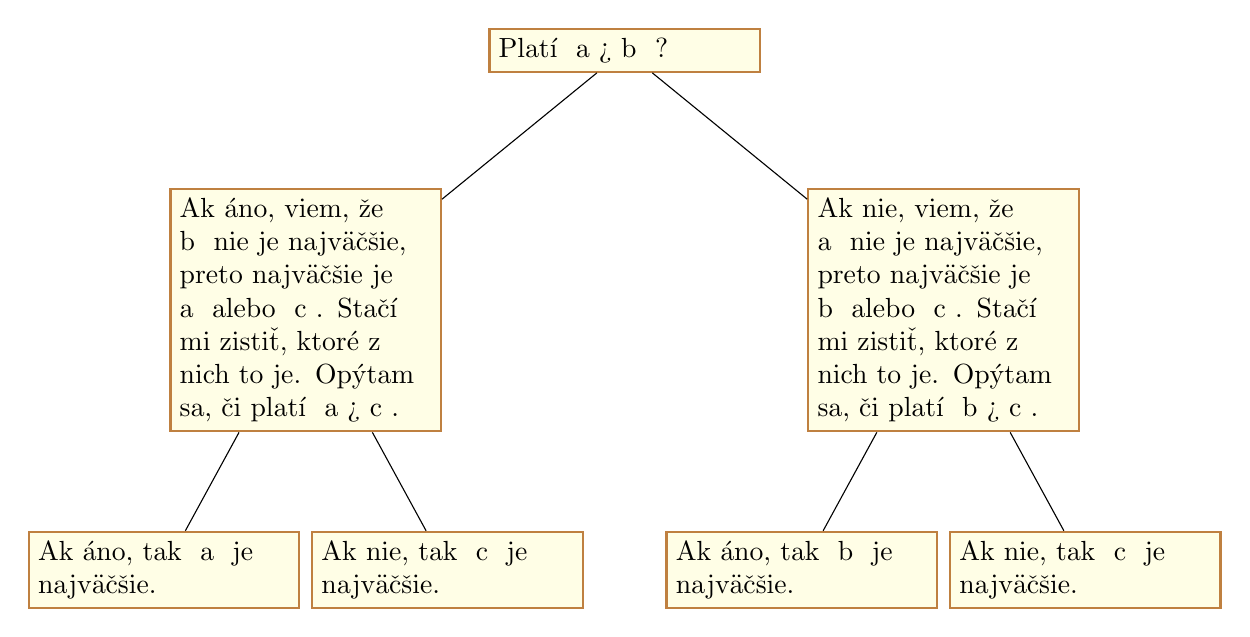
\begin{tikzpicture}[xscale=0.9,yscale=1.1]
  \tikzstyle{every node}=[text width=3.2cm,
  draw=brown, thick, fill=yellow!10]
  \tikzstyle{level 1}=[sibling distance=9cm]
  \tikzstyle{level 2}=[sibling distance=4cm]
  \node
  {Platí \prg~a > b~ ?} 
  [level distance =3cm] 
  child{
    node{Ak áno, viem, že \prg~b~ nie je najväčšie, preto 
    najväčšie je \prg~a~ alebo \prg~c~. Stačí mi zistiť, ktoré z nich to je. 
    Opýtam sa, či platí \prg~a > c~.}
    child{node{Ak áno, tak \prg~a~ je najväčšie.}}
    child{node{Ak nie, tak \prg~c~ je najväčšie. }}
  }
  child{
    node{Ak nie, viem, že \prg~a~ nie je najväčšie, preto 
    najväčšie je \prg~b~ alebo \prg~c~. Stačí mi zistiť, ktoré z nich to je. 
    Opýtam sa, či platí \prg~b > c~.}
    child{node{Ak áno, tak \prg~b~ je najväčšie.}}
    child{node{Ak nie, tak \prg~c~ je najväčšie. }}
  }
  ;
  \end{tikzpicture}


Toto viem zapísať do programu :

\begin{lstlisting}
#include <iostream>
using namespace std;
int main() {
    int a, b, c;
    cin >> a >> b >> c;
    if (a > b) {      
      if (a > c)
        cout << a;
      else
        cout << c;
    } else {
      if (b > c)
        cout << b;
      else
        cout << c;
    }
    cout << endl;
}
\end{lstlisting}


Tu som použil skrátený zápis: namiesto \prg~int a; int b; int c;~ môžem napísať
\prg~int a, b, c;~ a namiesto 

\begin{lstlisting}
cin >> a;  cin >> b;  cin >> c;
\end{lstlisting}

môžem písať
\prg~cin >> a >> b >> c;~ Tiež si si už asi všimol, že nezáleží na tom, ako
sú v texte programu medzery a riadky. Je rozumné mať text {\em odsadený} tak,
aby sa dal dobre čítať: každý príkaz na zvláštnom riadku a vnorené príkazy 
majú na začiatku riadku viac medzier, aby začínali viac vpravo. 
Rovnako je dobré nazvať premenné tak,
aby bolo z názvu jasné, čo je v nich uložené. 
Ale nie je to nutné. Aj toto\footnote{
  Program je zo súťaže \href{www.ioccc.org}{\nolinkurl{www.ioccc.org}} o 
  najnečitateľnejší C/C++ 
  program
  (\href{https://www.ioccc.org/2011/eastman/hint.html}{%
\nolinkurl{https://www.ioccc.org/2011/eastman/hint.html}}).}
je správny program, ale nie je ľahké zistiť, 
čo vlastne robí:

\vbox{
\begin{lstlisting}
#include <stdio.h>
#include <math.h>
#include <unistd.h>
#include <sys/ioctl.h>

             main() {
         short a[4];ioctl
      (0,TIOCGWINSZ,&a);int
    b,c,d=*a,e=a[1];float f,g,
  h,i=d/2+d%2+1,j=d/5-1,k=0,l=e/
 2,m=d/4,n=.01*e,o=0,p=.1;while (
printf("\x1b[H\x1B[?25l"),!usleep(
79383)){for (b=c=0;h=2*(m-c)/i,f=-
.3*(g=(l-b)/i)+.954*h,c<d;c+=(b=++
b%e)==0)printf("\x1B[%dm ",g*g>1-h
*h?c>d-j?b<d-c||d-c>e-b?40:100:b<j
||b>e-j?40:g*(g+.6)+.09+h*h<1?100:
 47:((int)(9-k+(.954*g+.3*h)/sqrt
  (1-f*f))+(int)(2+f*2))%2==0?107
    :101);k+=p,m+=o,o=m>d-2*j?
      -.04*d:o+.002*d;n=(l+=
         n)<i||l>e-i?p=-p
             ,-n:n;}}
\end{lstlisting}
}

\begin{uloha}
 Napíš program, ktorý načíta tri čísla a vypíše prostredné z nich.
\end{uloha}

\begin{uloha}
  Napíš program, ktorý načíta číslo mesiaca (1 pre január, 2 pre február, atď.)
  a vypíše číslo ročného obdobia 
  (1 pre jar, 2 pre leto, 3 pre jeseň a 4 pre zimu).
\end{uloha}

